\documentclass{beeper}

\usepackage{fontawesome}
\usepackage{etoolbox}
\usepackage{textcomp}
\usepackage[nodisplayskipstretch]{setspace}
\usepackage{xspace}
\usepackage{verbatim}
\usepackage{multicol}
\usepackage{soul}
\usepackage{attrib}

\usepackage{amsmath,amssymb,amsthm}

\usepackage[linesnumbered,commentsnumbered,ruled,vlined]{algorithm2e}
\newcommand\mycommfont[1]{\footnotesize\ttfamily\textcolor{blue}{#1}}
\SetCommentSty{mycommfont}
\SetKwComment{tcc}{ \# }{}
\SetKwComment{tcp}{ \# }{}

\usepackage{siunitx}

\usepackage{tikz}
\usepackage{pgfplots}
\usetikzlibrary{decorations.pathreplacing,calc,arrows.meta,shapes,graphs}

\setmainfont{Open Sans Light}
\usefonttheme{serif}

\makeatletter
\patchcmd{\beamer@sectionintoc}{\vskip1.5em}{\vskip0.5em}{}{}
\makeatother

% Math stuffs
\newcommand{\Z}{\mathbb{Z}}
\newcommand{\R}{\mathbb{R}}
\newcommand{\N}{\mathbb{N}}
\newcommand{\lcm}{\text{lcm}}
\newcommand{\Inn}{\text{Inn}}
\newcommand{\Aut}{\text{Aut}}
\newcommand{\Ker}{\text{Ker}\ }
\newcommand{\la}{\langle}
\newcommand{\ra}{\rangle}

\newcommand{\yournewcommand}[2]{Something #1, and #2}

\newenvironment{question}[1]{\par\textbf{Question #1.}\par}{}

\newcommand{\pmidg}[1]{\parbox{\widthof{#1}}{#1}}
\newcommand{\splitslide}[4]{
    \noindent
    \begin{minipage}{#1 \textwidth - #2 }
        #3
    \end{minipage}%
    \hspace{ \dimexpr #2 * 2 \relax }%
    \begin{minipage}{\textwidth - #1 \textwidth - #2 }
        #4
    \end{minipage}
}

\newcommand{\frameoutput}[1]{\frame{\colorbox{white}{#1}}}

\newcommand{\tikzmark}[1]{%
\tikz[baseline=-0.55ex,overlay,remember picture] \node[inner sep=0pt,] (#1)
{\vphantom{T}};
}

\newcommand{\braced}[3]{%
    \begin{tikzpicture}[overlay,remember picture]
        \draw [thick,decorate,decoration={brace,raise=1ex,amplitude=4pt},blue] (#2.south west-|T1.south west) -- node[anchor=west,left,xshift=-1.8ex,text=olive]{#3} (#1.north west-|T1.south west);
    \end{tikzpicture}
}

\title{Matrix Cryptographic Key Infrastructure}
\author{Sumner Evans}
\institute{Beeper (Automattic)}
\date{21 September 2024}

\begin{document}

\begingroup
\def\insertframenumber{\relax}
\begin{frame}
    \titlepage

    \note[item]{
        Hello, my name is Sumner, I'm a software engineer at Automattic working
        on Beeper.
    }
    \note[item]{
        End-to-end encryption is one of the things which \textbf{brought me to
        Matrix}, and I'm sure that it's one of the factors that brought many of
        you to Matrix as well.
    }
    \note[item]{
        However, Matrix's user experience with cryptography is often confusing.
    }
    \note[item]{
        I mainly \textbf{blame the other chat networks} for their incompetence.
    }
    \note[item]{
        Most other chat networks \textbf{don't provide} any
        cryptographically-guaranteed security and privacy.
    }
    \note[item]{
        Of the ones that do, most do so in a way that \textbf{does not truly
        leave the user in control of their keys}.
    }
    \note[item]{
        Only a few networks, namely Signal, truly leave the user in control, and
        their UX is arguably worse than Matrix.
    }
    \note[item]{
        In this talk, my goal is to discuss the \textbf{cryptographic key
        \textit{infrastructure} in Matrix}.
    }
    \note[item]{
        What do I mean by ``infrastructure''? I mean all of the features which
        \textbf{support key sharing and identity verification}, but don't
        actually themselves provide security.
    }
    \note[item]{
        You can think of this talk as discussing the ``UX layer of cryptography
        in Matrix''. None of the things that I'm going to discuss are strictly
        necessary for ensuring secure communication, but without them, Matrix'
        UX would be horrible.
    }
\end{frame}
\endgroup

\begin{frame}{Why Cryptography?}
    Matrix uses cryptography for two main purposes:\pause

    \begin{enumerate}
        \item \textbf{Message Security} --- only the people who are part of the
            conversation should be allowed to view messages of the conversation.
            \pause
        \item \textbf{Identity} --- verifying that a user or device is who they
            say they are.
    \end{enumerate}

    \note[item]{
        Now, let's discuss what Matrix even uses cryptography for. There are two
        main purposes...
    }

    \note[item]{
        The first is \textbf{message security}. We only want the people who are
        part of the conversation to be able to read the messages in the
        conversation.
    }
    \note[item]{
        As an additional benefit of how Matrix achieves this, encrypted messages
        \textbf{cannot be tampered with} by a \textbf{man-in-the-middle} actor
        without the receiving party knowing.
    }

    \note[item]{
        The second reason for using cryptography in Matrix is \textbf{identity}
        verification. We want to know that a specific device or user is who they
        say they are.
    }
    \note[item]{
        Note that one of the most important uses for identity verification is
        verifying your own devices so you can share keys with them.
    }
\end{frame}

\begin{frame}{Big Picture}
    \includegraphics[width=\textwidth]{images/overview}

    \note[item]{
        Let's take a look at what we are going to talk about today. This diagram
        shows \textbf{how those core features are implemented} as well as the
        infrastructure that supports them.
    }
    \note[item]{
        I know, it's pretty overwhelming. But don't worry, we are \textbf{going
        to go step-by-step} through this. By the end of the talk you should have
        an understanding of what each part of this diagram means.
    }
    \note[item]{
        It's probably too small to read, but I want to start by
        \textbf{orienting ourselves} to what's going on in this diagram, and we
        will zoom in later.
    }
    \note[item]{
        You can see that there are \textbf{two users represented} in the
        diagram: Bob on the top and Alice on the bottom. The diagram is
        \textbf{focused on how} the Megolm session created by Alice Device 1 is
        \textbf{shared} to Bob and to Alice's Device 2.
    }
    \note[item]{
        You'll notice that the diagram is color-coded.
        \begin{itemize}
            \item Red nodes represent data that does not leave the device.
            \item Green nodes represent data is public and can be shared with
                the server and other users.
            \item Orange nodes represent data that can be shared with trusted
                parties, or with members of the same Matrix room.
            \item Blue and purple nodes represent cryptographic operations.
        \end{itemize} 
    }
\end{frame}

\begin{frame}{Big Picture: Message Security}
    \includegraphics[width=\textwidth]{images/message-security}

    \note[item]{
        It's important that we \textbf{don't loose sight} of the reason for all
        of this infrastructure. Highlighted in \textbf{orange}, we have the
        \textbf{core of Matrix security: the Megolm session}.
    }
    \note[item]{
        We aren't going to discuss this in detail today. I \textbf{wrote an
        article} about Megolm which you can find on my blog if you want to learn
        more. I'll provide a link at the end of the talk.
    }
    \note[item]{
        For now, the only thing you need to know about it is that it's what is
        used to \textbf{encrypt and decrypt messages}.
    }
    \note[item]{
        The Megolm session needs to be \textbf{shared} with all the devices that
        Alice wants to be \textbf{able to read her messages}. So it needs to be
        shared to
        \begin{itemize}
            \item the devices of \textbf{other users} in the Matrix room (in
                this case Bob)
            \item as well as \textbf{her other devices}.
        \end{itemize}
    }
    \note[item]{
        All of the rest of the infrastructure in this diagram is to facilitate
        transferring that Megolm session, or verifying that a device should in
        fact have access to that Megolm session.
    }
\end{frame}

\begin{frame}{Big Picture: Identity}
    \includegraphics[width=\textwidth]{images/identity-overview}

    \note[item]{
        Let's move on to identity. The highlighted parts of the diagram provide
        a cryptographic way to verify that a device belongs to a particular
        user.
    }
    \note[item]{
        There are actually two pieces here...
    }
\end{frame}

\begin{frame}{Big Picture: Identity: Device Verification}
    \includegraphics[width=\textwidth]{images/identity-device-verification}

    \note[item]{
        Here we have the infrastructure necessary for determining if we
        \textbf{trust another device for our own user}.
    }
\end{frame}

\begin{frame}{Big Picture: Identity: User Verification}
    \includegraphics[width=\textwidth]{images/identity-user-verification}

    \note[item]{
        And here we have the infrastructure necessary for determining if we
        \textbf{trust another user and their devices}.
    }
\end{frame}

\begin{frame}{Big Picture: The Other Stuff}
    \includegraphics[width=\textwidth]{images/other-stuff}

    \note[item]{
        So what is all of the other stuff? That is the \textbf{infrastructure}
        for sharing the Megolm session around to other devices and users.
    }
\end{frame}

\begin{frame}{Big Picture: The Other Stuff: To-Device}
    \includegraphics[width=\textwidth]{images/other-stuff-to-device}

    \note[item]{
        For example, in this arrow represents \textbf{sending} the Megolm
        session via \textbf{Olm-encrypted to-device messages}.
    }
\end{frame}

\begin{frame}{Big Picture: The Other Stuff: Key Backup}
    \includegraphics[width=\textwidth]{images/other-stuff-key-backup}

    \note[item]{
        This \textbf{lower-right section} of the diagram represents \textbf{key
        backup} which allows you to \textbf{backup} your keys to the
        \textbf{server} and restore from your other devices.
    }
\end{frame}

\begin{frame}{Big Picture: The Other Stuff: Secure Secret Storage and Sharing}
    \includegraphics[width=\textwidth]{images/other-stuff-ssss}

    \note[item]{
        And over here on the \textbf{left} we have the infrastructure necessary
        for \textbf{storing secrets} on the \textbf{server} encrypted by a
        \textbf{recovery code}.
    }
\end{frame}

\begin{frame}{Big Picture}
    \includegraphics[width=\textwidth]{images/overview}

    \note[item]{
        So, that's a \textbf{quick overview} of this diagram.
    }

    \note[item]{
        \textbf{Before} we dive deeper into the \textbf{details} of the diagram,
        we need to \textbf{discuss} some basic \textbf{cryptography primitives}.
    }

    \note[item]{
        Then we will \textbf{break down} the diagram into manageable pieces.
    }
\end{frame}

\section{Cryptography Crash Course}
\note{
    I will try and explain the cryptography primitives in \textbf{simple terms}.
    It's \textbf{not} going to be \textbf{mathematically rigorous}, but will
    focus on the \textbf{functionality} that each cryptographic primitive
    provides.
}

\begin{frame}{Encryption: Symmetric vs Asymmetric}
    There are two main categories of encryption schemes:

    \begin{itemize}
        \item \textbf{Symmetric} --- both \textbf{the encryptor and the
            decryptor share the same key} and that key is used in both the
            encryption and decryption of the message
            \pause
        \item \textbf{Asymmetric} --- \textbf{the encryptor needs the public
            key, and the decryptor needs the private key} and the encryptor
            encrypts the message with the public key, and the private key is
            required to decrypt the message
    \end{itemize}

    \note[item]{
        Let's start with \textbf{encryption}. Encryption allows us to make a
        message that can only be read by another user who has the key.
    }
    \note[item]{
        \textit{Read slide}
    }
    \note[item]{
        There are a few variants of asymmetric encryption schemes. Matrix uses
        elliptic-curves for its asymmetric encryption needs.
    }
\end{frame}

\begin{frame}{Asymmetric Signatures}
    In addition to providing encryption, asymmetric encryption schemes also
    provide \textbf{signatures}.
    \pause

    Signing uses the \textit{private} key, and anyone who possesses the
    \textit{public} key can verify the signature.

    \note[item]{
        Only the private key can create a valid signature.
    }

    \note[item]{
        This is the opposite of encryption where we use the public key to
        encrypt, and the private key to decrypt.
    }
\end{frame}

\begin{frame}{Hashes and HMAC}
    A \textbf{cryptographic hash function} is a one-directional function which
    takes an arbitrarily large set of data and produces a unique fixed-size
    output (called the hash).
    \pause

    \textbf{Given the same data, a hash function will always return the same
    output.}
    \pause

    This allows us to verify that the data did not change in transit (for
    example, by a malicious actor).
    \pause

    Hashes are vulnerable to \textbf{metadata attacks}. To prevent these, we use
    HMAC which adds a secret key to the hash.

    \note[item]{
        \textit{Read slide to last bullet}
    }
    \note[item]{
        If you \textbf{hash} the \textbf{same message} multiple times, you will
        receive the \textbf{same value}, and an attacker could use this
        information to deduce the \textbf{frequency} of certain
        \textbf{messages} being sent.
    }
    \note[item]{
        \textit{Read last bullet}
    }
    \note[item]{
        \textbf{How} the \textbf{key} is \textbf{added} is an implementation
        detail that is \textbf{not relevant}. All you need to know is that HMAC
        prevents metadata attacks.
    }
\end{frame}

\begin{frame}{Key-Derivation Functions (HKDF)}
    Sometimes, we want to turn a small key into a larger key (or set of larger
    keys).

    \note[item]{
        \textit{Read first bullet}
    }
    \note[item]{
        For example, we might want to \textbf{``stretch''} a 32-byte
        \textbf{shared secret} into a key and IV for AES and a key for HMAC
        which would be 80 bytes in total.
    }
    \note[item]{
        \textit{Read rest of slide}
    }

    \textbf{Key-Derivation Functions (KDFs)} are used to do this.
    \pause

    Matrix uses HKDF which uses HMAC for the key derivation process.
\end{frame}

\begin{frame}{Diffie-Hellman Key Exchanges}
    Often, we need a way to share keys with both the sending and receiving
    parties across an unsecured channel.
    \note[item]{
        \textit{Read first bullet}... such as the internet.
    }
    \note[item]{
        We \textbf{can share} keys securely \textbf{in-person}, but that is very
        \textbf{impractical}.

        That's where the \textbf{Diffie-Hellman (DH) Key Exchange} method comes
        in.
    }
    \pause

    \textbf{Diffie-Hellman} is a method for using public-key cryptography to
    facilitate keysharing.

    \note[item]{
        \textit{Read second bullet slide}
    }
    \note[item]{
        Since Matrix uses elliptic-curve cryptography, the \textbf{specific
        variant} of Diffie-Hellman that Matrix uses is ECDH (the elliptic curve
        variant).

        I'm not going to discuss the actual mathematical mechanism behind ECDH
        as it's quite complex and not relevant to understanding how Matrix uses
        ECDH. However, it is essential to understand the main feature it
        provides:
    }

    \[
        \textbf{ECDH}(A_{private}, B_{public}) = \textbf{ECDH}(B_{private}, A_{public}) = K_{shared}.
    \]

    \note[item]{
        \textit{Read equation}
    }
    \note[item]{
        In this equation, we have two public/private keypairs: \(A\) and \(B\).
    }
    \note[item]{
        If we have \textbf{either one} of the \textbf{private} keys and the
        \textbf{other public key}, we can \textbf{generate} the same
        \textbf{shared secret}.
    }
    \note[item]{
        \textit{Go through example of what to do if you have \(A_{private}\) vs
        having \(B_{private}\)}
    }

    \note[item]{
        We will get the \textbf{same value} out of ECDH \textit{regardless of
        which private key you have}. You only \textbf{need} the other
        \textbf{public} key, and those are \textbf{public} keys that can be
        spread around like butter.
    }
\end{frame}

\begin{frame}{Big Picture}
    \includegraphics[width=\textwidth]{images/overview}

    \note[item]{
        Let's go \textbf{back to the big picture} now. Recall that the
        \textbf{blue} and \textbf{purple} nodes represent \textbf{cryptographic
        operations}.
    }
    \note[item]{
        All these \textbf{nodes} are one of the operations that we discussed.
    }
    \note[item]{
        \textit{Point out a couple of HKDF, AES, ECDH, HMAC}
    }
    \note[item]{
        Now, let's discuss \textbf{how} these are \textbf{composed} together to
        provide \textbf{features} within Matrix.
    }
\end{frame}

\section{Sharing Keys}
\note{
    We're going to start by discussing how we get \textbf{keys} from \textbf{one
    device to another}. This process is generally called \textbf{``key
    sharing''}.
}

\begin{frame}{Big Picture: Message Security}
    \includegraphics[width=\textwidth]{images/message-security}

    \note[item]{
        Remember, what we are \textbf{trying to share} is the \textbf{Megolm
        key} because that's what \textbf{encrypts and decrypts} the
        \textbf{messages}.
    }

    \note[item]{
        There are \textbf{two} ways to share these: \textbf{encrypted olm
        events} and \textbf{key backup}.
    }
\end{frame}

\begin{frame}{Encrypted Olm Events}
    \includegraphics[width=\textwidth]{images/other-stuff-to-device}

    \note[item]{
        \textbf{Encrypted Olm events} are represented by the \textbf{arrows}
        highlighted in \textbf{red}. They are sent via \textbf{to-device}
        messages which allow you to send messages to specific devices (rather
        than rooms).
    }

    \note[item]{
        Let's zoom in to see what's going on.
    }
\end{frame}

\begin{frame}{Encrypted Olm Events}
    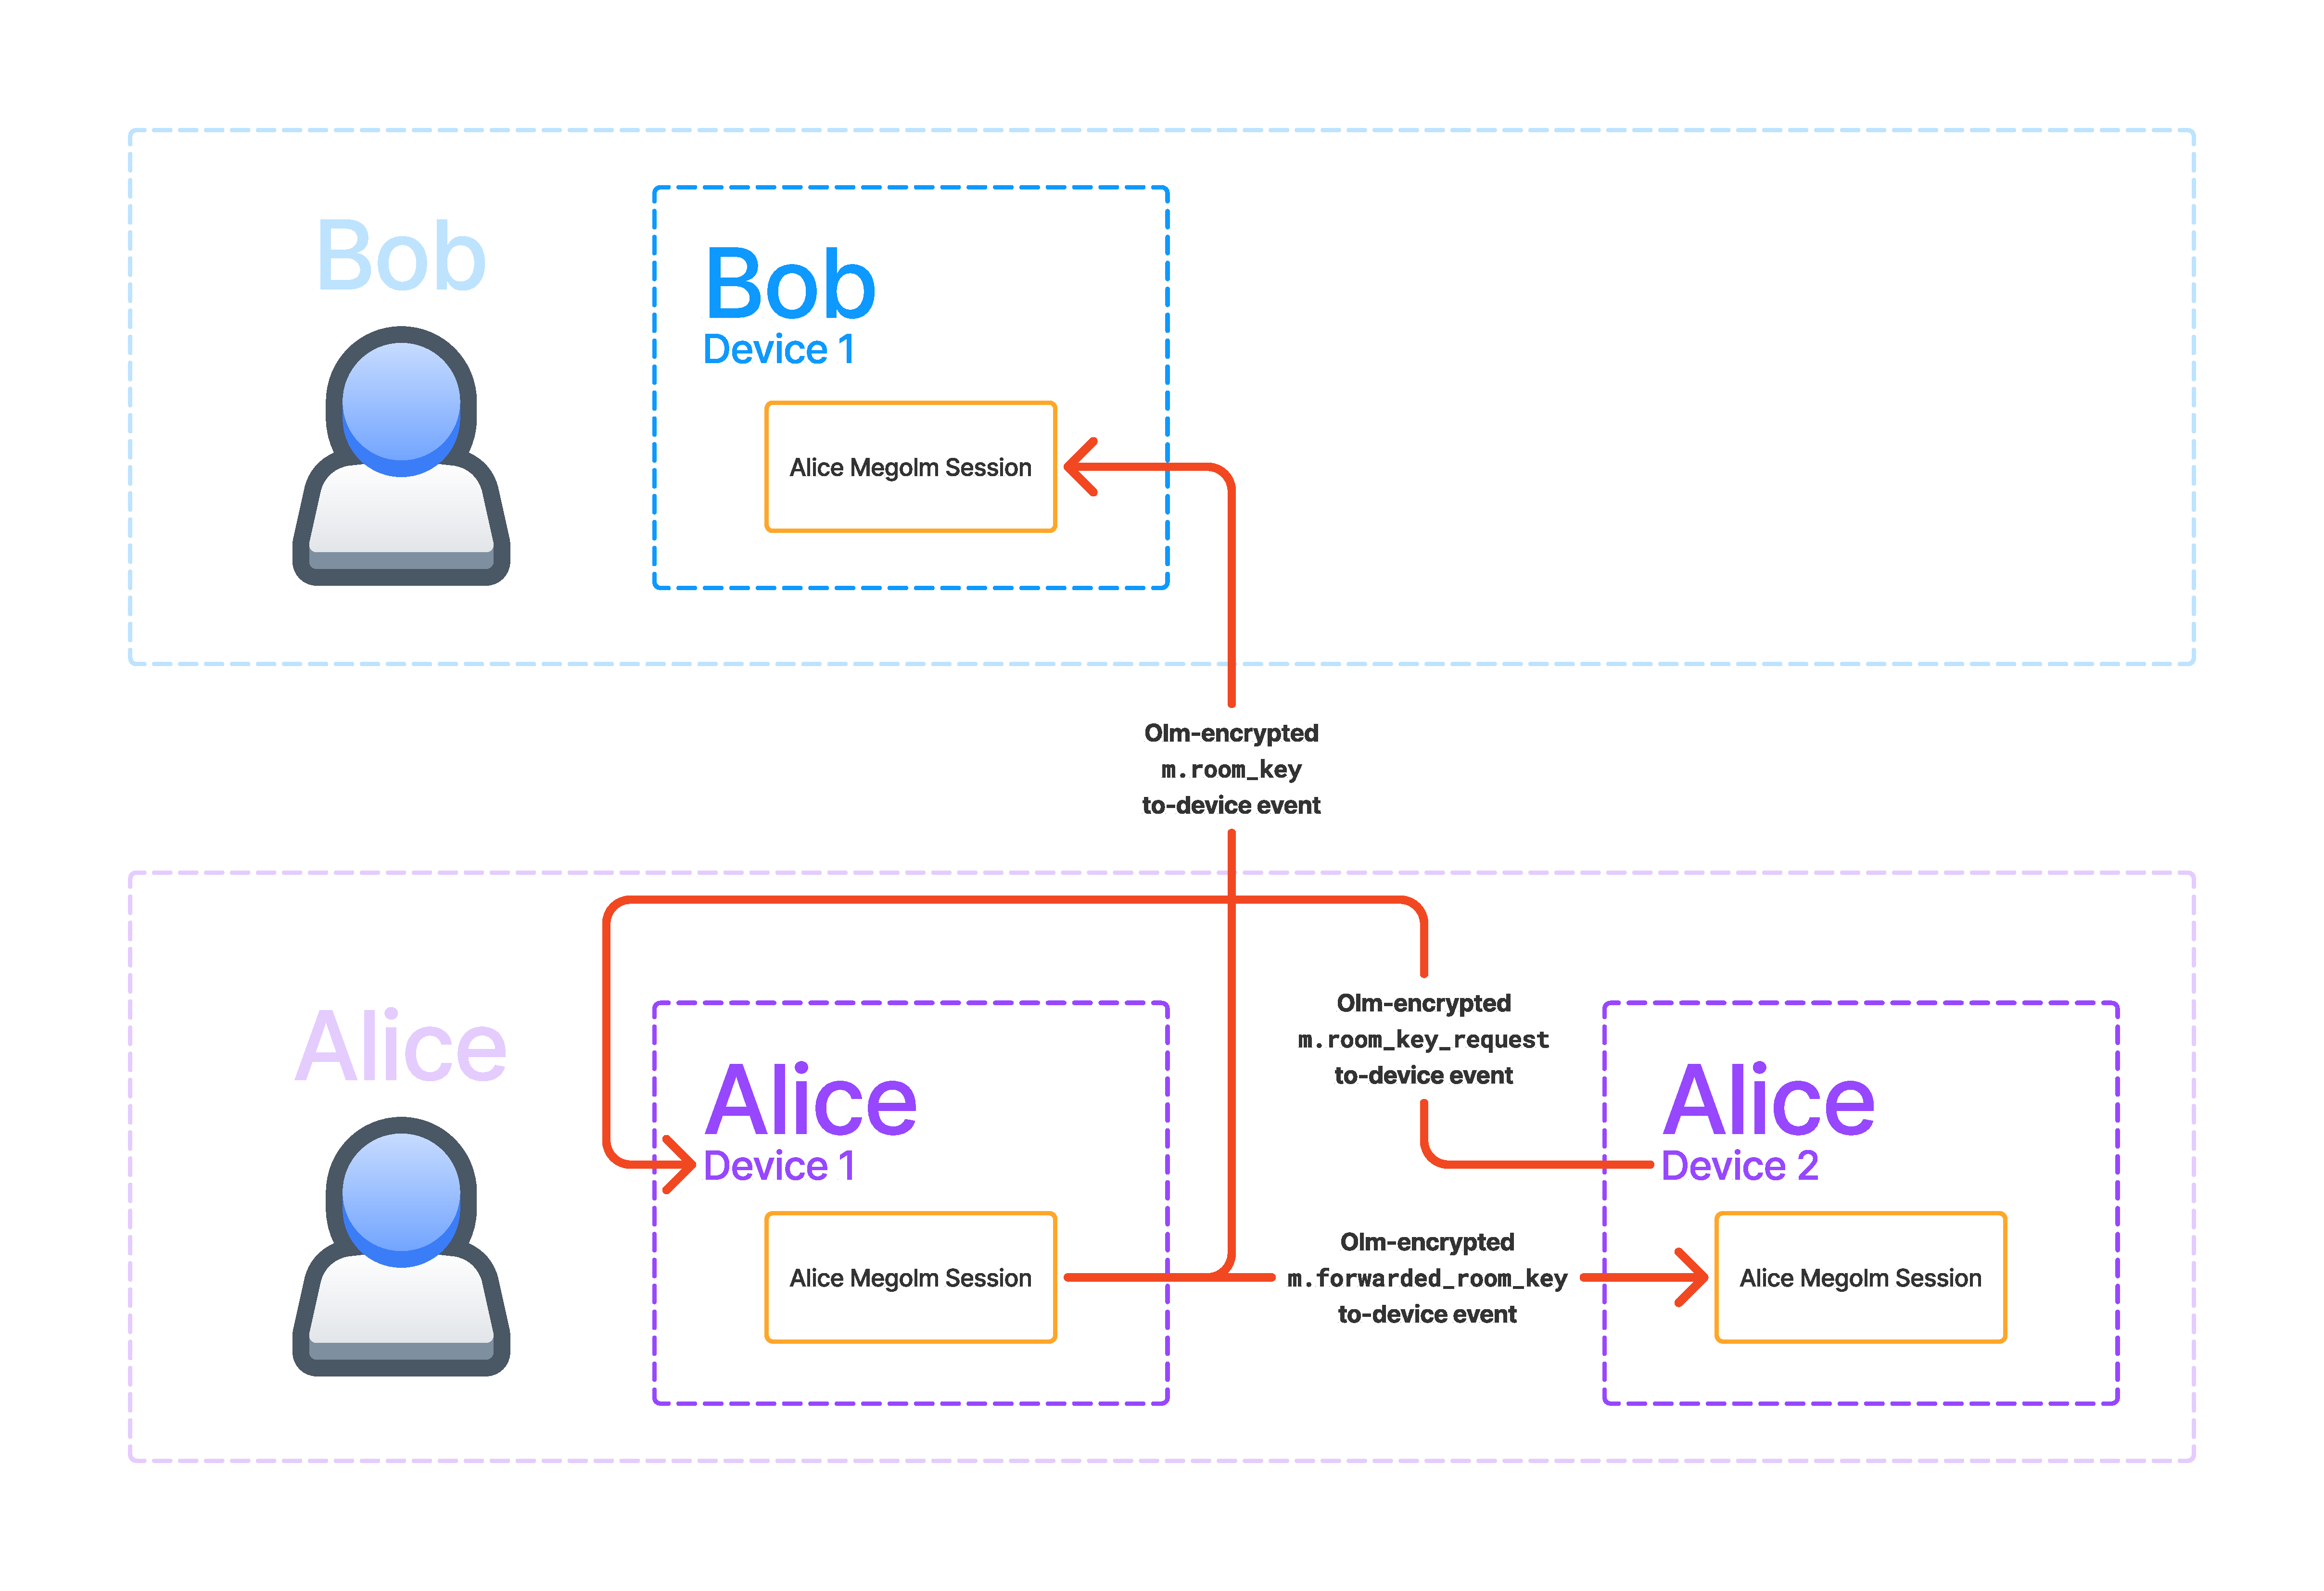
\includegraphics[width=\textwidth]{images/to-device-zoomed}

    \note[item]{
        I got rid of all the irrelevant nodes
    }
    \note[item]{
        You can see that we can \textbf{send} keys to \textbf{other users'
        devices} via \texttt{m.room\_key} events.
    }
    \note[item]{
        And actually we use \texttt{m.room\_key} events to send keys to our
        \textbf{own devices} as well.
    }
    \note[item]{
        We can also \textbf{request keys} by sending
        \texttt{m.room\_key\_request} events to our \textbf{own verified
        devices} and the other devices can respond using
        \texttt{m.forwarded\_room\_key} events. We will talk about how we know a
        device is verified later.
    }

    \note[item]{
        I'm not going to discuss how Olm encryption works. It's already been
        covered many times since it's basically just the Signal double-ratchet
        algorithm.
    }

    \note[item]{
        For our purposes, it's \textbf{sufficient} to know that we can
        \textbf{send keys securely} to \textbf{other users' devices} and our
        \textbf{own devices} via these events.
    }

    \note[item]{
        This seems great, why do we have anything else?
    }

    \note[item]{
        Well, \textbf{new logins} are the issue. Say Alice just \textbf{logged
        in} on \textbf{Device 2} and finished verification.

        \begin{itemize}
            \item If Device 1 is \textit{online}, she can send key requests to
                Device 1 and Device 1 can respond.

                This \textbf{works}, but there will likely be a \textbf{lot of
                keys} to request. \textbf{Every user} in \textbf{every encrypted
                room} has diffrent keys.

                This will make \textbf{Device 1} do a \textbf{lot of work} to
                send back all the keys.

                On \textbf{mobile devices}, keysharing \textbf{can't} really be
                done in the \textbf{background}, \textbf{especially} on
                \textbf{iOS}.

                Even on \textbf{desktop} devices, it's still a lot of
                \textbf{work} to \textbf{process} a \textbf{flood} of key
                \textbf{requests}.
            \item But it's \textbf{even worse} if Device 1 is \textit{offline}.
                In that case, Alice's key \textbf{requests} will \textbf{never
                be answered}.
        \end{itemize}
    }
\end{frame}

\begin{frame}{Key Backup}
    \includegraphics[width=\textwidth]{images/other-stuff-key-backup}

    \note[item]{
        This ss where \textbf{key backup} comes into play. Key backup allows us
        to \textbf{store keys} on the \textbf{server}, and \textbf{restore} them
        from our \textbf{other devices} even if your \textbf{other devices} are
        \textbf{offline} or \textbf{inaccessible}.
    }

    \note[item]{
        Let's zoom in and see what's going on.
    }
\end{frame}

\begin{frame}{Key Backup}
    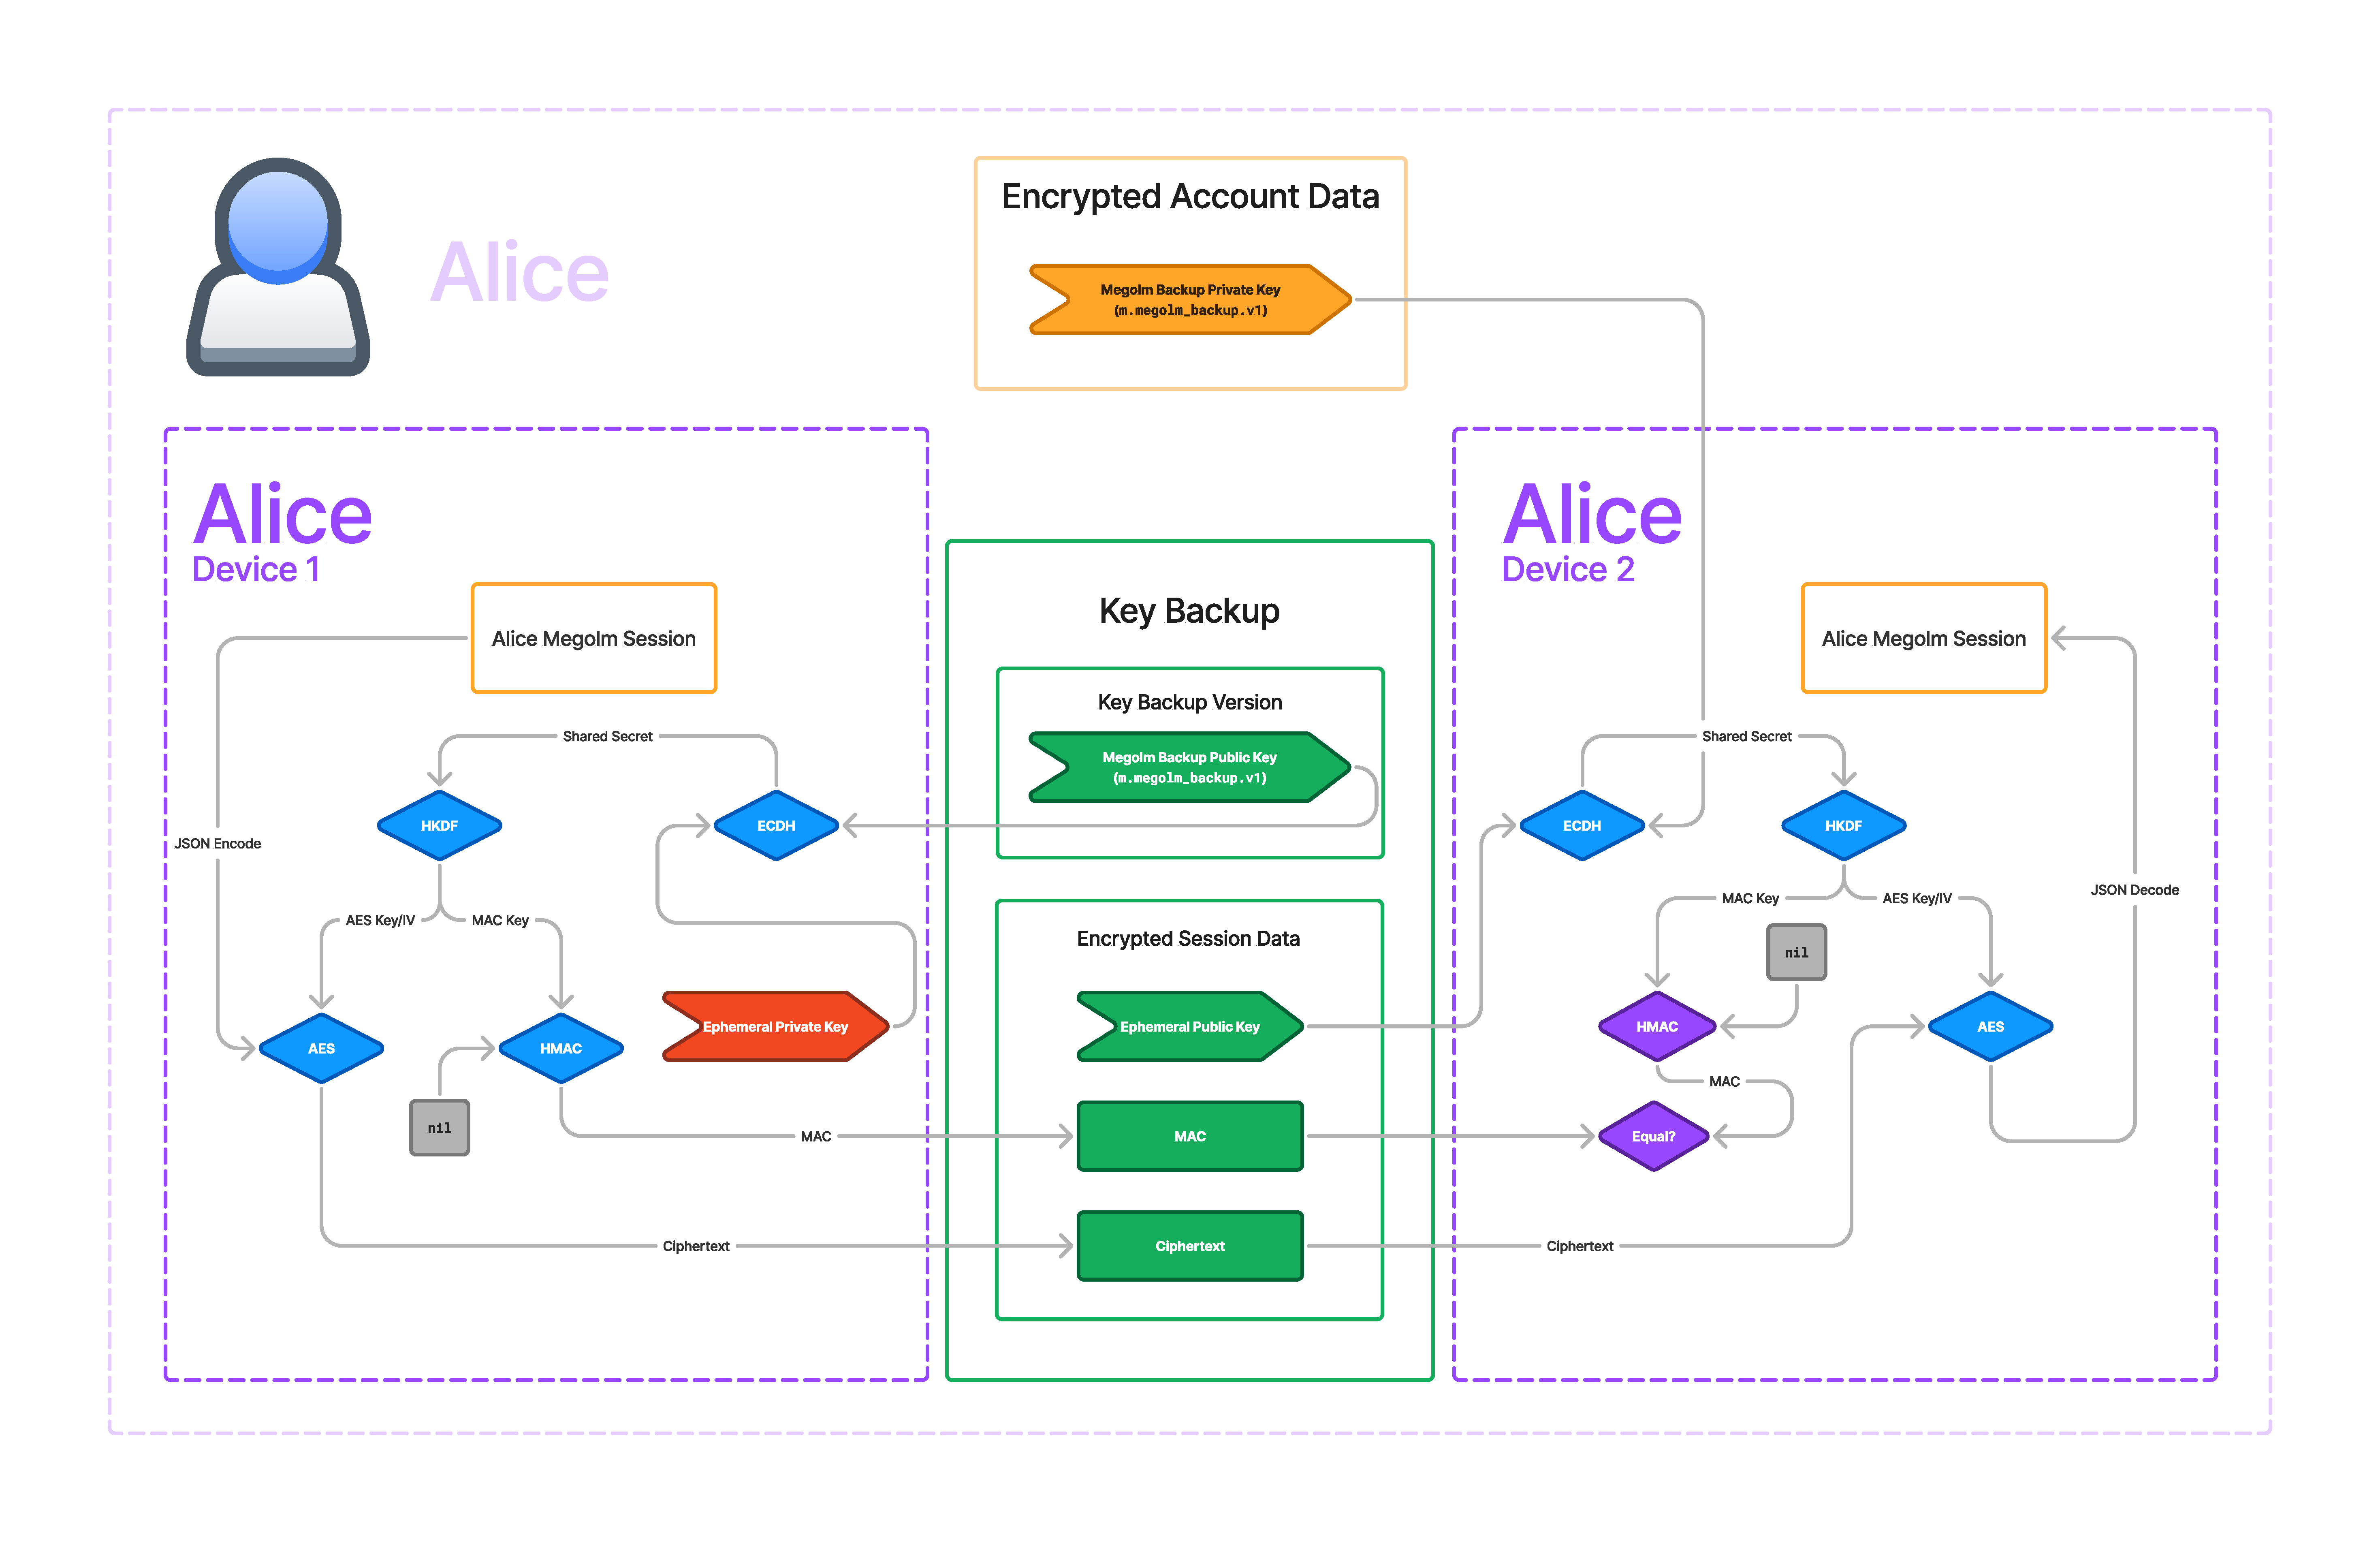
\includegraphics[width=\textwidth]{images/key-backup-zoomed}

    \note[item]{
        In the \textbf{middle} here we have the ``key backup'' in
        \textbf{green}. Key backup is is \textbf{stored} on the \textbf{server}.
    }
    \note[item]{
        In this diagram, we're trying to get the Megolm key \textbf{from}
        Alice's \textbf{Device 1} to her \textbf{Device 2}, so \textbf{left to
        right}.
    }
    \note[item]{
        There are \textbf{two pieces} to key backup:

        \begin{itemize}
            \item the \textbf{key backup version} which includes the
                \textbf{backup public key}.
            \item the \textbf{encrypted session data} for \textbf{each} of the 
                backed-up Megolm \textbf{sessions}.
        \end{itemize}
    }

    \note[item]{
        Let's discuss how this works.
    }

    \note[item]{
        The \textbf{first thing} to note is that \textbf{AES} is used on
        \textbf{both sides} to \textbf{encrypt} and \textbf{decrypt} the
        \textbf{Megolm session}. \textbf{Only} the \textbf{encrypted} version is
        \textbf{stored} on the \textbf{server}.
    }
    \note[item]{
        But, \textbf{AES} needs a \textbf{key} and \textbf{initial vector}.
        Where do we get that from? Well, we \textbf{get it from HKDF}.
    }
    \note[item]{
        HKDF \textbf{requires a key as well}, so where do we get that from?
    }

    \note[item]{That comes from a call to ECDH.}

    \note[item]{
        Note that \textbf{everything so far} is \textbf{the same on both the
        encrypting and decrypting sides!}
    }

    \note[item]{
        Recall that \textbf{ECDH} requires a \textbf{private key}, and the
        \textbf{other public key}.
    }
\end{frame}

\begin{frame}{Key Backup}
    \begin{center}
    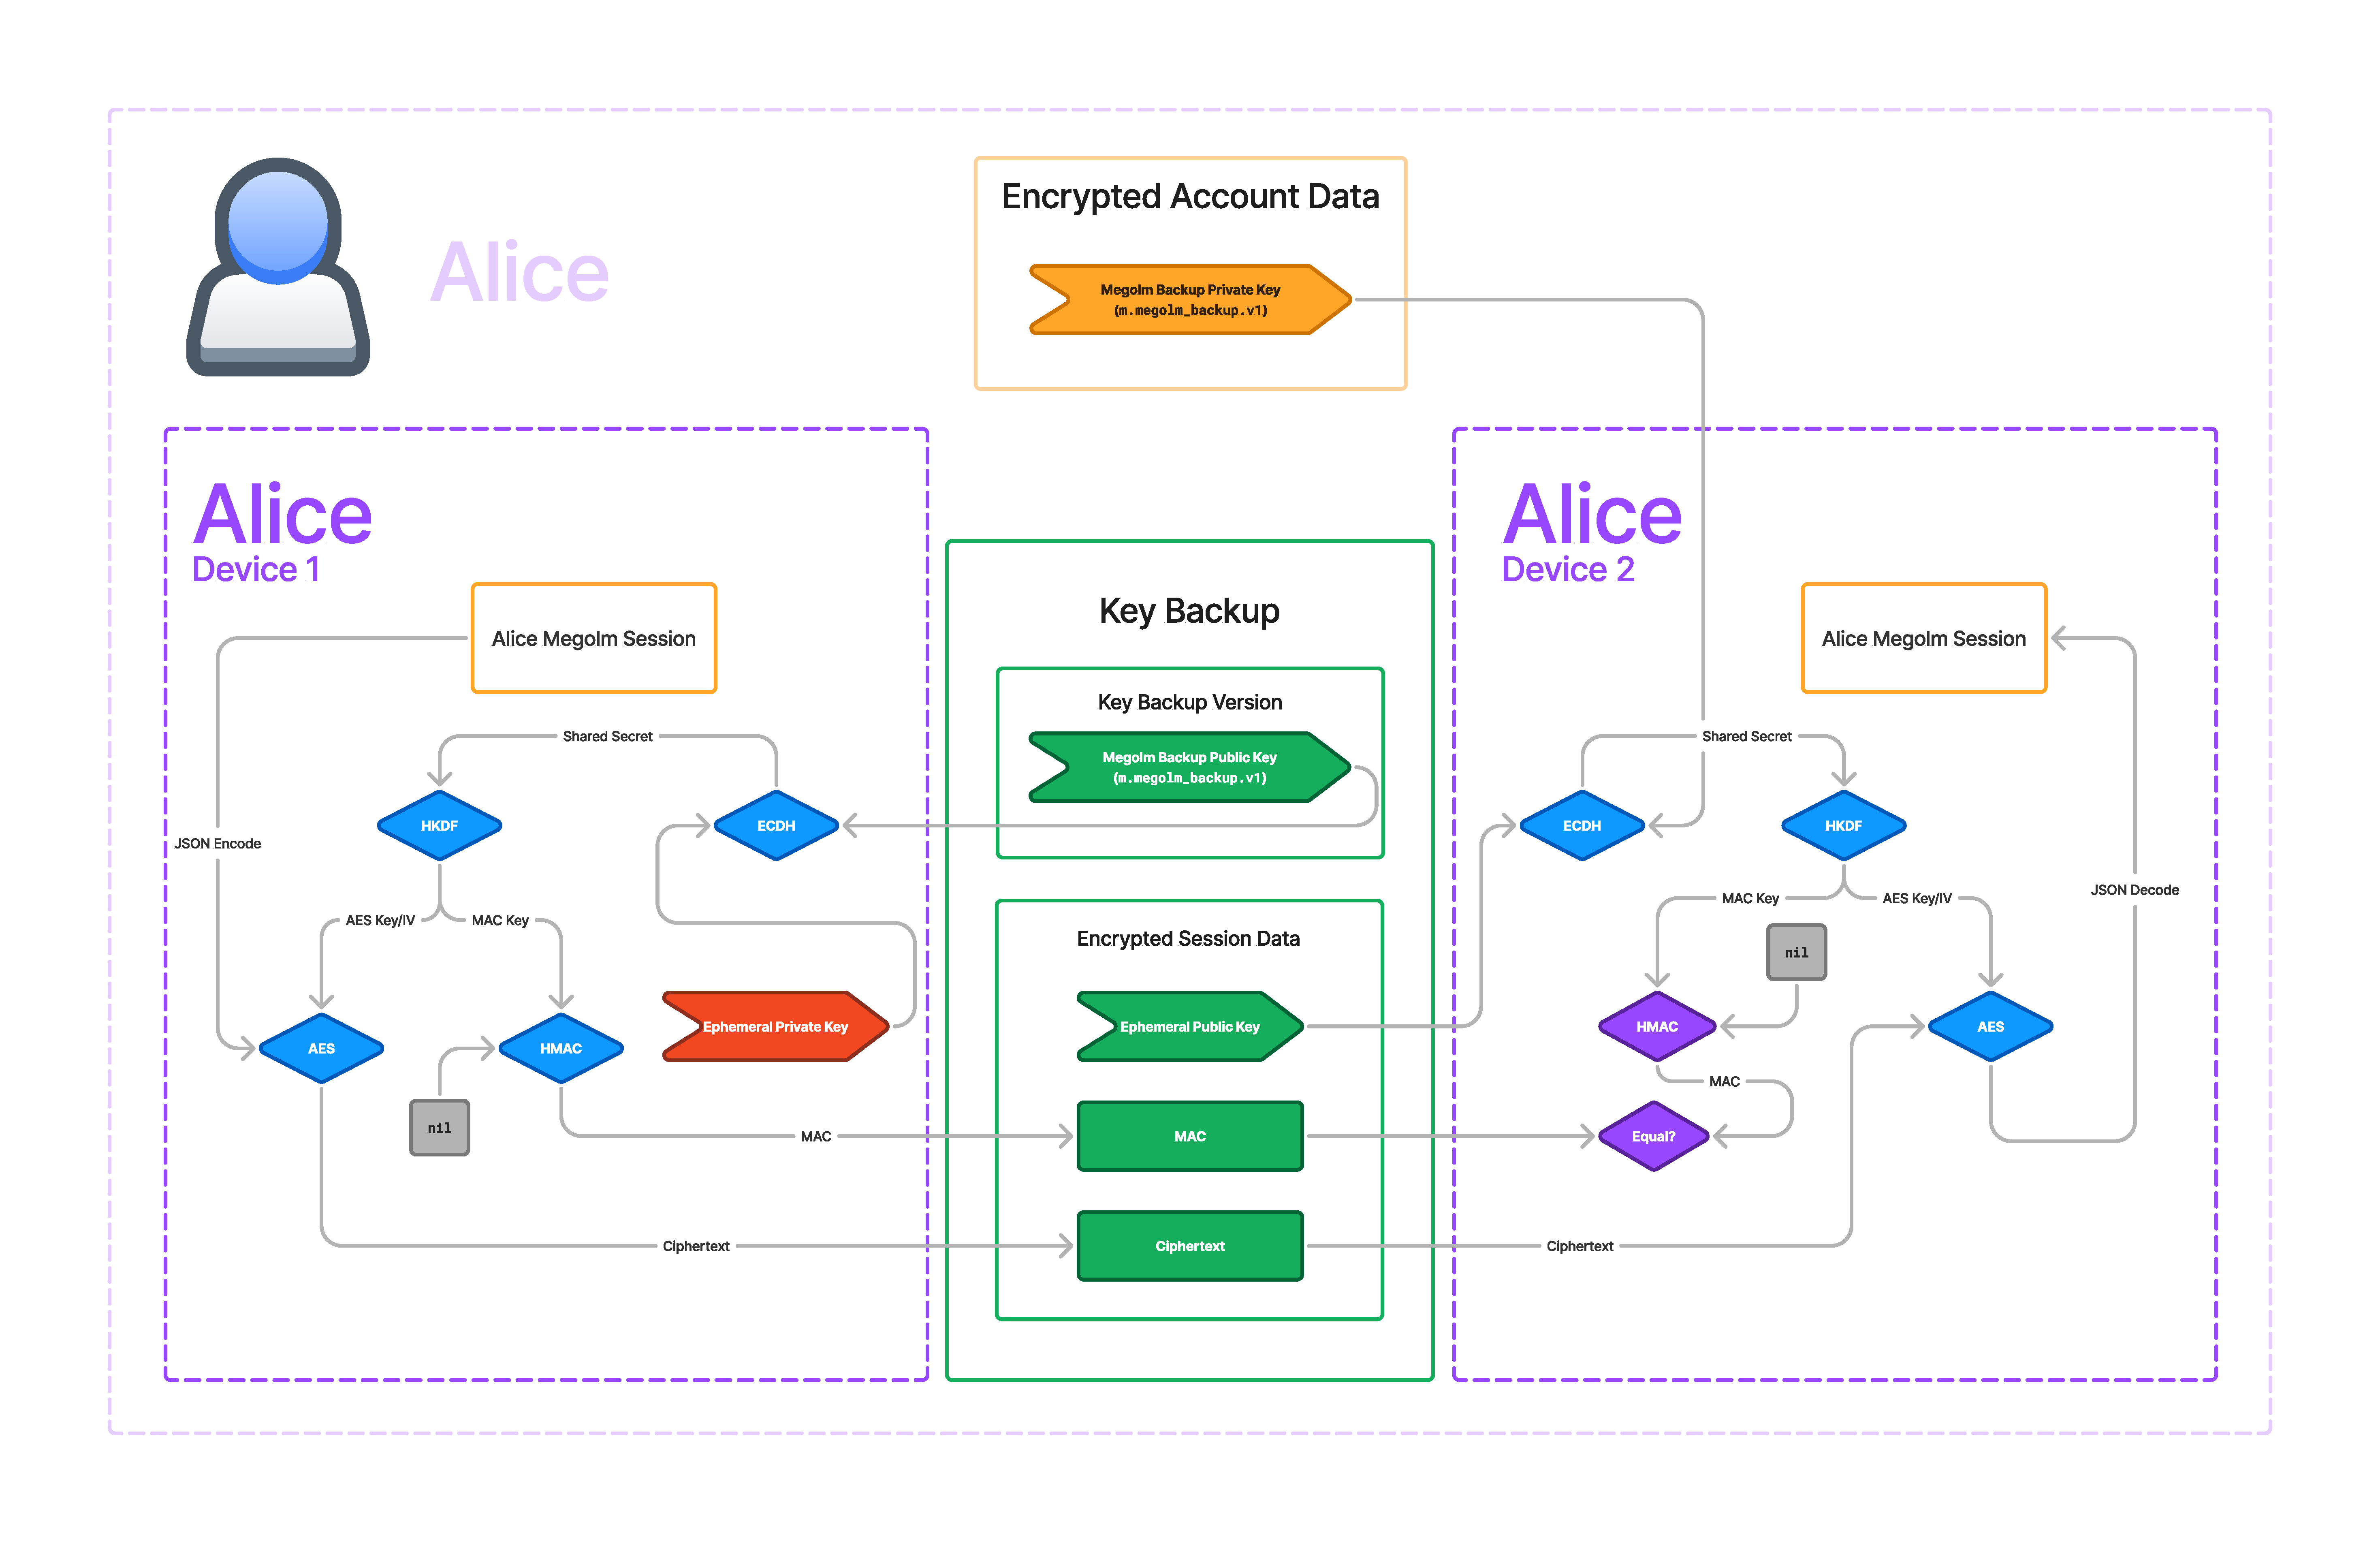
\includegraphics[width=0.9\textwidth]{images/key-backup-zoomed}
    \end{center}

    \vspace{-2em}

    \[\textbf{ECDH}(A_{private}, B_{public}) = \textbf{ECDH}(B_{private}, A_{public}) = K_{shared}\]

    \note[item]{
        Remember this formula? If you have \textbf{either private key}, we just
        \textbf{need} the \textbf{other public key} to get the same value from
        ECDH.
    }

    \note[item]{
        So where do we get the \(A\) and \(B\) keypairs from?
        \begin{itemize}
            \item The \textbf{first keypair} is the \textbf{Megolm backup
                keypair}. The \textbf{public key} is stored in the \textbf{key
                backup version}. The \textbf{private key} is a secret stored on
                the \textbf{user's device}.
            \item The \textbf{second keypair} is the \textbf{ephemeral keypair}.
                A \textbf{new keypair} gets created for \textbf{each} backed up
                session. It's \textbf{ephemeral because} the \textbf{private}
                part is be \textbf{discarded} immediately \textbf{after the
                encryption} is done. The \textbf{public key} is stored in the
                \textbf{encrypted session data}.
        \end{itemize}
    }

    \note[item]{
        This is where the \textbf{sides diverge}.
    }

    \note[item]{
        \begin{itemize}
            \item The \textbf{encrypting} side gets its \textbf{private key}
                from the \textit{ephemeral keypair}.

                And it uses the \textbf{Megolm backup public key} as its public
                key.
            \item The \textbf{decrypting} side gets its \textbf{private key}
                from the \textbf{Megolm backup private key}.

                And it uses the \textbf{ephemeral public key} as its public key.
        \end{itemize}
    }

    \note[item]{
        Critically you \textbf{must have} the \textbf{Megolm backup private key}
        to \textbf{decrypt} the key \textbf{backup}.
    }

    \note[item]{
        For \textbf{each Megolm session} that we \textbf{back up} in key backup,
        we \textbf{store} the \textbf{ephemeral public key} and the
        \textbf{ciphertext} from AES together in the \textbf{encrypted session
        data} object.
    }
\end{frame}

\begin{frame}{Key Backup}
    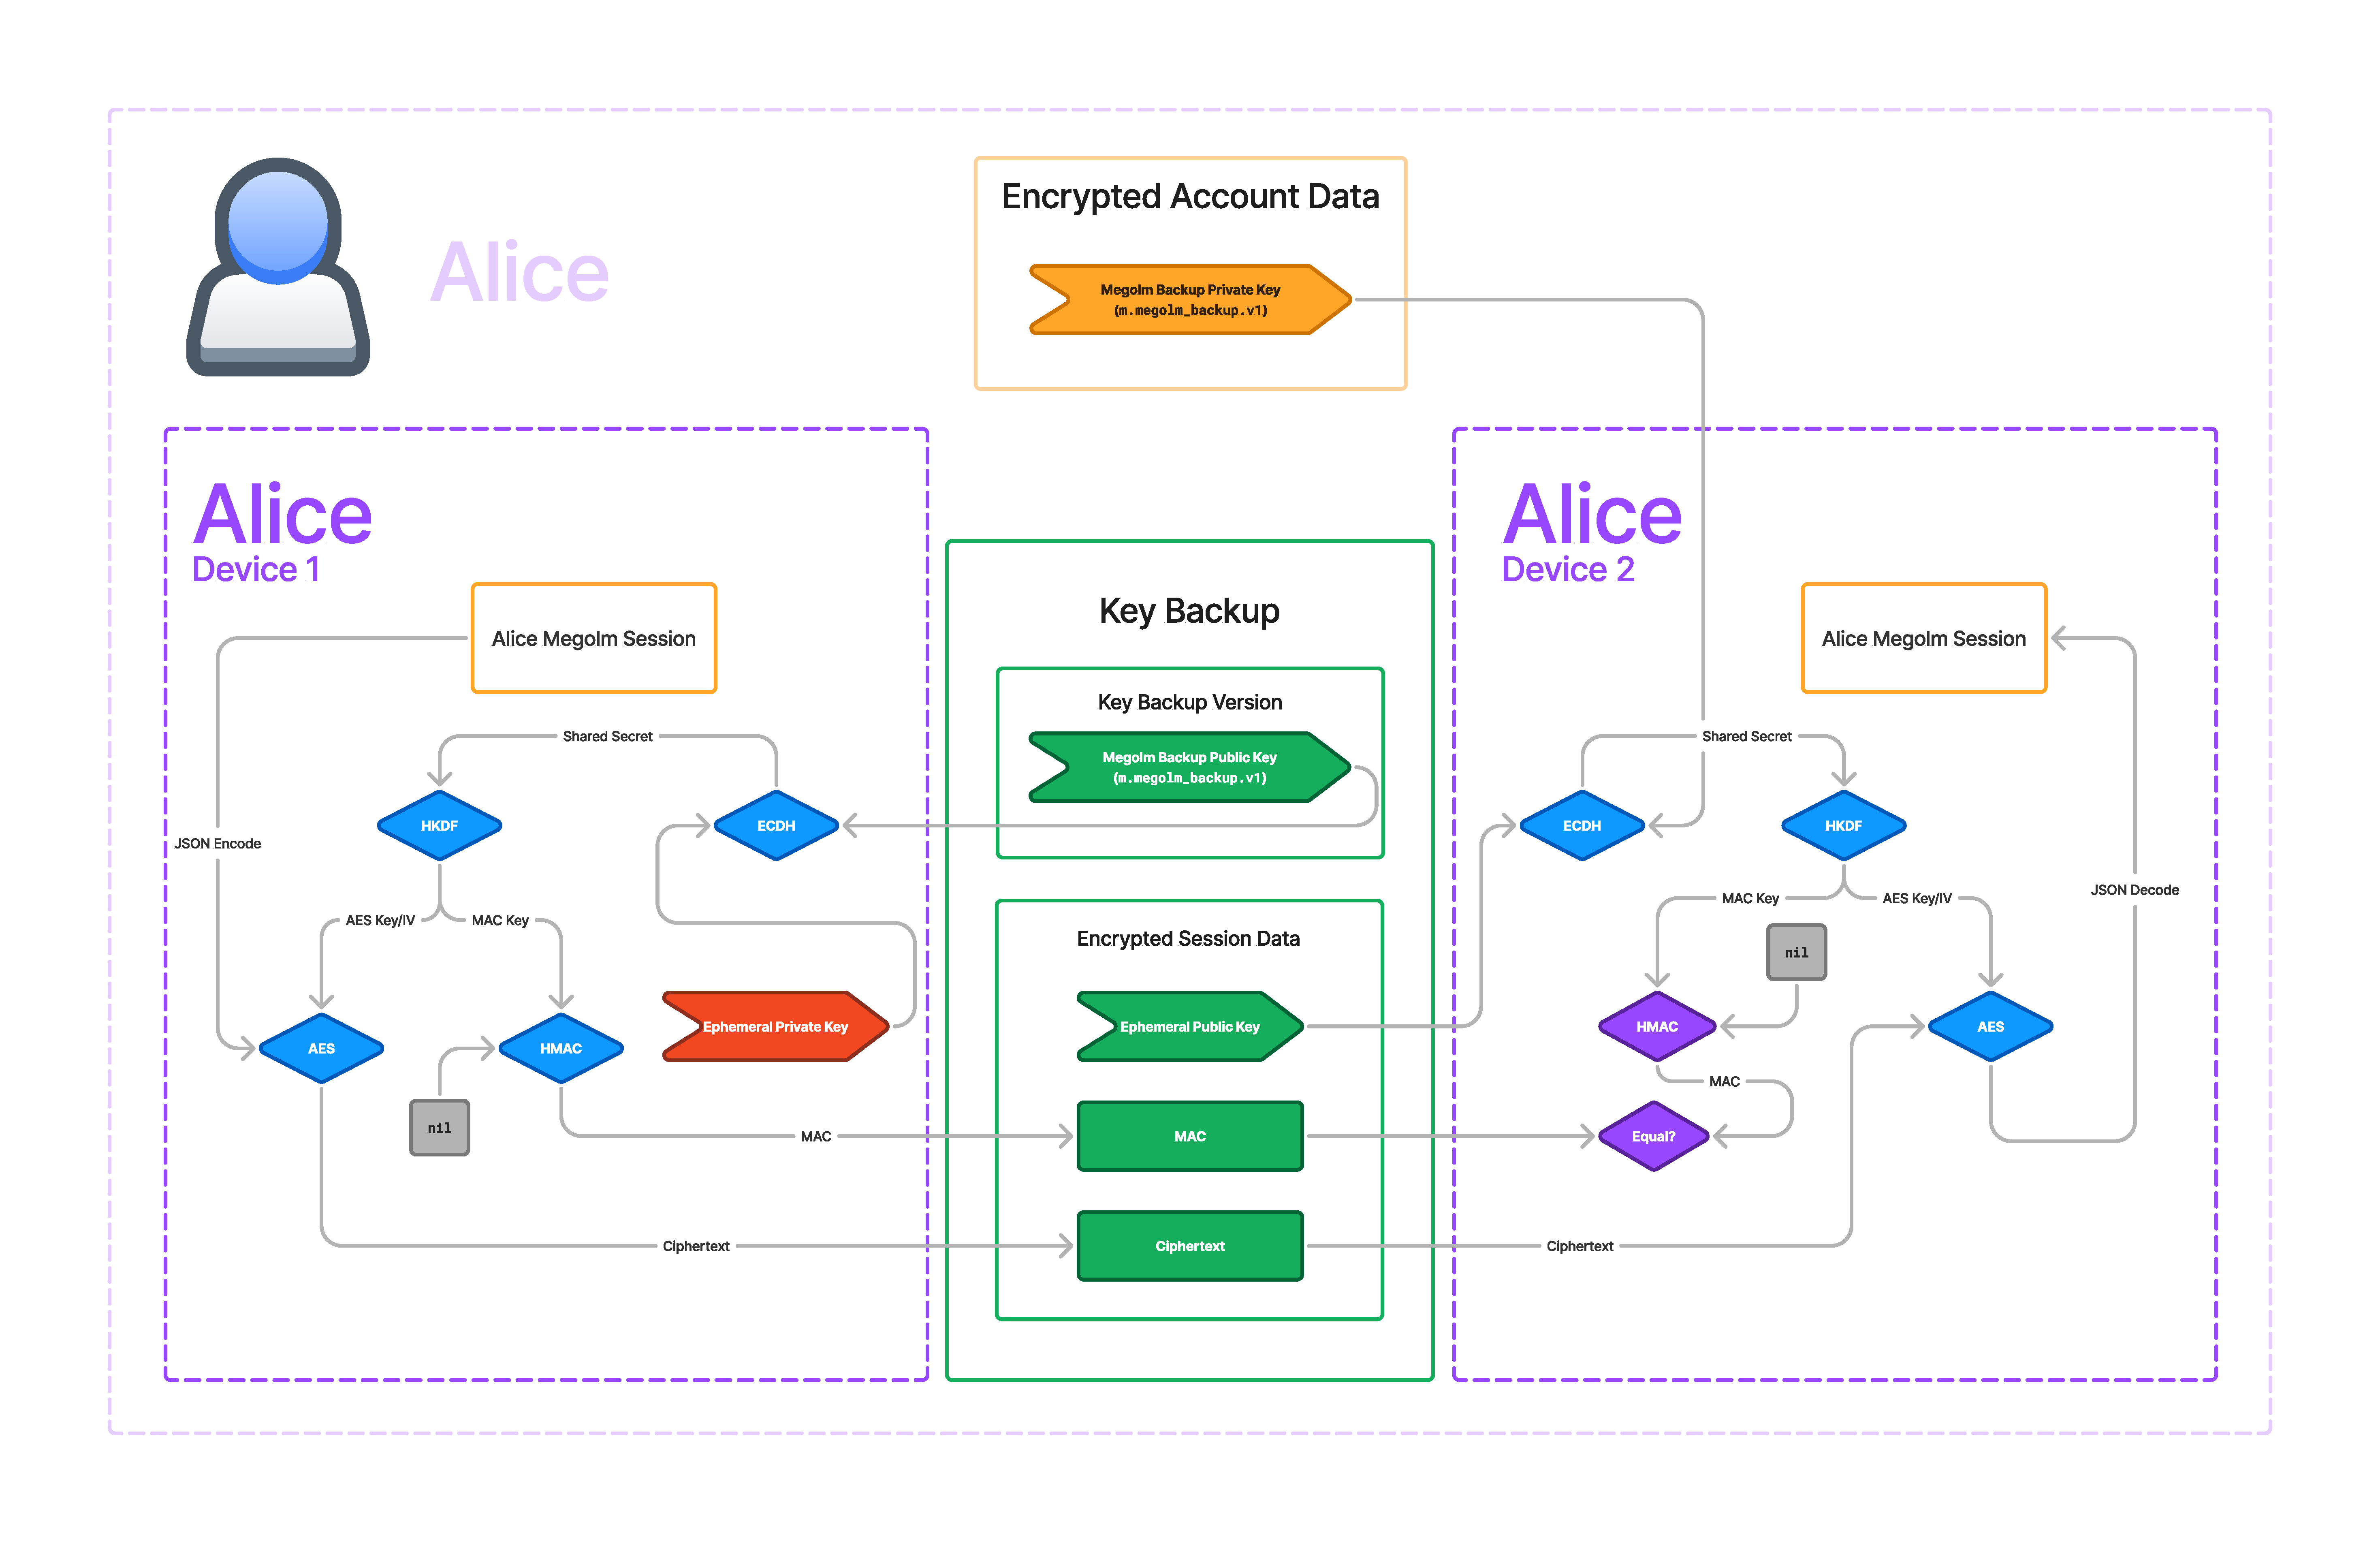
\includegraphics[width=\textwidth]{images/key-backup-zoomed}

    \note[item]{
        But there's \textbf{another item} that we store in this object: the
        \textbf{MAC}.
    }

    \note[item]{
        A \textbf{MAC} is a \textbf{Message Authentication Code}. It's basically
        just a \textbf{hash} of the \textbf{ciphertext} that we use to
        \textbf{verify} that it hasn't been \textbf{tampered} with by a
        \textbf{malicious} or just straight up \textbf{incompetent} party.
    }

    \note[item]{
        We use \textbf{HMAC} to \textbf{generate the MAC} and \textbf{avoid
        metadata attacks}. Recall that HMAC requires a key.
    }
    \note[item]{
        Conviniently, we are \textbf{already using HKDF} to generate the
        \textbf{AES key and initial vector}, so we can just use the \textbf{same
        key derivation} to get the \textbf{HMAC key}.
    }

    \note[item]{
        What \textit{should} happen is that we \textbf{pass} the
        \textbf{ciphertext} into \textbf{HMAC}. However, the original
        implementation in \textbf{libolm failed to do this} correctly and
        instead just passed an \textbf{empty buffer}, and it has been de-facto
        spec ever since.
    }

    \note[item]{
        So, the \textbf{MAC} is \textbf{not really useful} at all in its
        \textbf{current state}. I'm hoping that a future version of the spec
        fixes this.
    }
\end{frame}

\section{Device Verification}
\note{
    Now, let's discuss \textbf{device verification}.
}

\begin{frame}{Who Can We Send Keys To?}
    \includegraphics[width=\textwidth]{images/to-device-own-user}

    \note[item]{
        Let's go back to the big picture and notice these \textbf{arrows} that
        represent \textbf{requesting keys} from our \textbf{own devices} and
        \textbf{forwarding} them back.
    }

    \note[item]{
        Earlier I said that we \textbf{only} want to \textbf{forward} keys to
        our \textbf{verified} devices?
    }

    \note[item]{
        Now, we are going to discuss how \textbf{verification status} is
        determined.
    }

    \note[item]{
        The answer is...
    }
\end{frame}

\begin{frame}{Signatures}
    \includegraphics[width=\textwidth]{images/identity-device-verification}

    \note[item]{
        \textbf{Signatures!}
    }

    \note[item]{
        Let's zoom in on this part.
    }

\end{frame}

\begin{frame}{Signatures}
    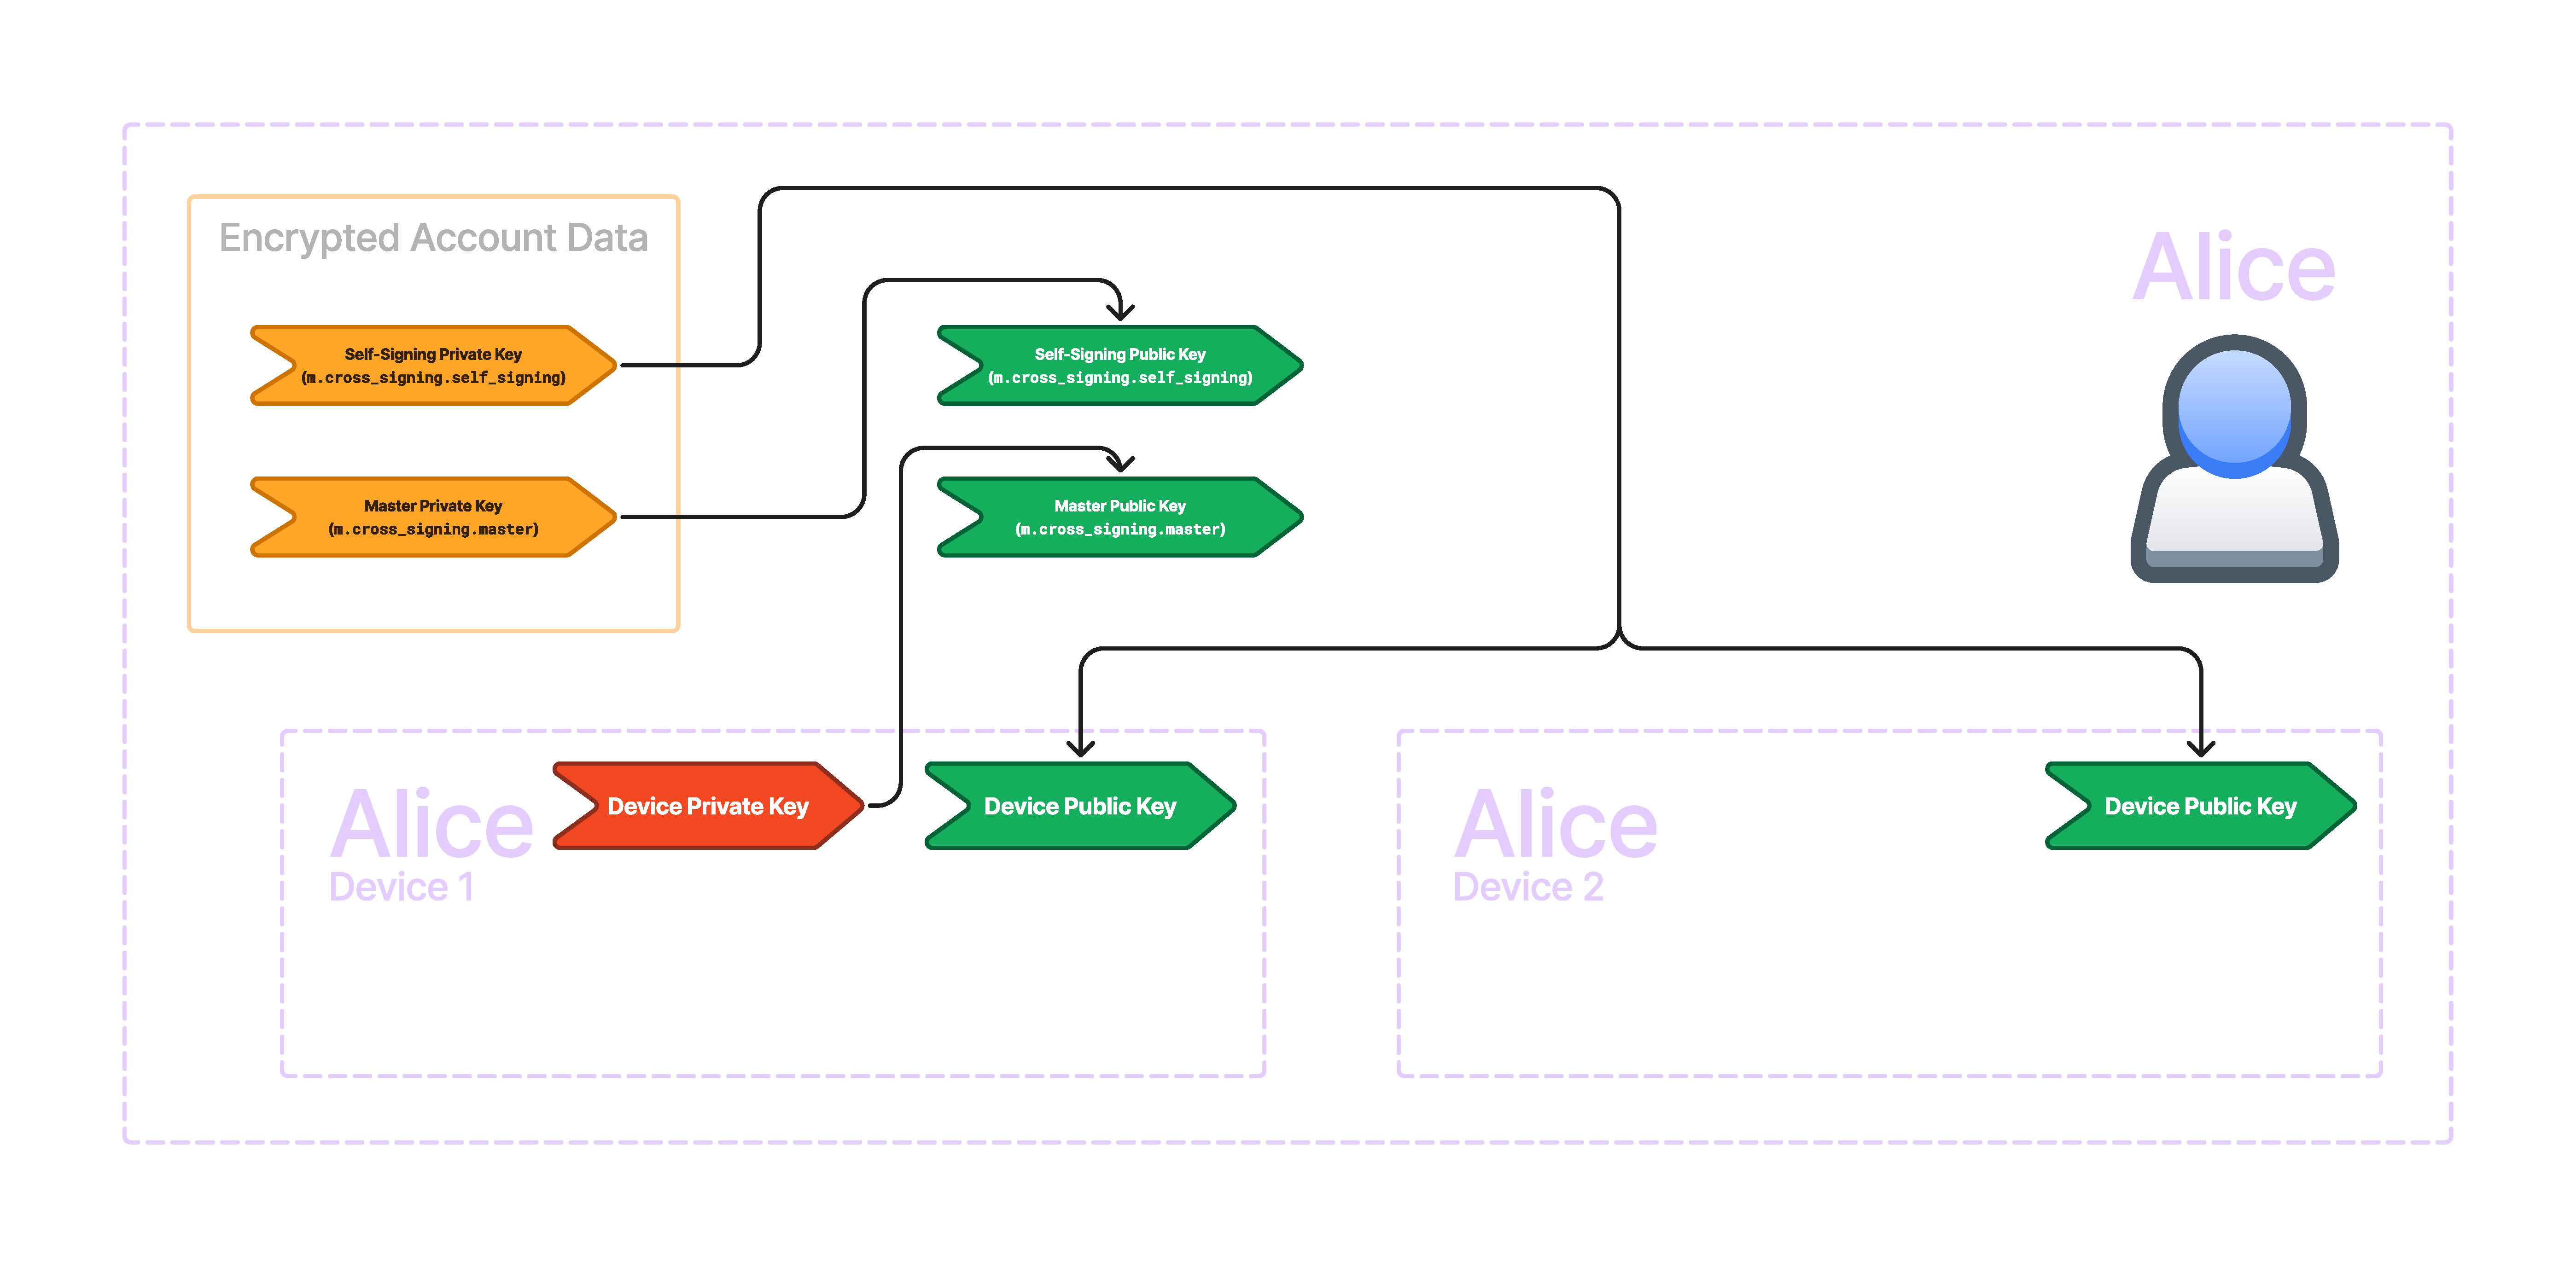
\includegraphics[width=\textwidth]{images/identity-device-verification-zoomed}

    \note[item]{
        Remember, \textbf{asymmetric signatures} can only be \textbf{created} by
        the \textbf{private} key, and anyone who possesses the \textbf{public}
        key can \textbf{verify} the signature.
    }

    \note[item]{
        In Matrix, each device has a \textbf{device keypair}. The
        \textbf{public} key is an \textbf{identifier} for the device.
    }

    \note[item]{
        To \textbf{verify} a device, we \textbf{sign} the \textbf{device public
        key}.
    }

    \note[item]{
        Often, we call this process \textbf{trusting} a key. We trust the key by
        \textbf{creating a signature} for it.
    }
    \note[item]{
        We \textbf{can} use our own \textbf{device private key} to
        \textbf{directly trust} the \textbf{other device key}.
    }
    \note[item]{
        But that is \textbf{inconvenient}. When we \textbf{log in} a \textbf{new
        device}, all our \textbf{other devices} will need to \textbf{make a
        signature for the new device}, and the \textbf{new device} will have to
        \textbf{make a signature for all the existing devices}!
    }

    \note[item]{
        So, we introduce a \textbf{new user-wide key} called the
        \textbf{``self-signing key''} because it \textbf{signs} our \textbf{own
        devices}.
    }

    \note[item]{
        We use the \textbf{self-signing} key to \textbf{sign the device keys}
        but \textbf{how} do we know if we should \textbf{trust} the
        \textbf{self-signing key?}
    }

    \note[item]{
        That's where the \textbf{master key} comes in. The master key
        \textbf{signs} the \textbf{self-signing key}.
    }

    \note[item]{
        We then \textbf{trust} the master key by \textbf{signing} it with our
        \textbf{device private key}.
    }

    \note[item]{
        This creates a \textbf{chain of trust}.

        The \textbf{device private key} signs the \textbf{master public key}
        which corresponds to the \textbf{master private key}.

        The \textbf{master private key} signs the \textbf{self-signing public
        key} which corresponds to the \textbf{self-signing private key}.

        And the \textbf{self-signing private key} signs \textbf{all} of the
        \textbf{device public keys}.
    }

    \note[item]{
        This allows us to \textbf{trust} a \textbf{single key} (in this case,
        the \textbf{master key}) and then through the \textbf{chain of trust},
        we can trust \textbf{all} of our \textbf{own devices}.
    }
\end{frame}

\section{User Verification}
\note{
    Sometimes, we want to \textbf{trust a user} so that we know that all of the
    \textbf{devices on their account} are \textbf{under their control}.
}

\begin{frame}{Additional Identity Verification}
    \includegraphics[width=\textwidth]{images/identity-user-verification}

    \note[item]{
        If a \textbf{new device is logged in}, we will know if they control the
        device if they have \textbf{signed} it.
    }
    \note[item]{
        If some \textbf{malicious actor} logged in a new device, they would
        \textbf{not} be able to \textbf{sign} it, and we would know the
        \textbf{other user} has been \textbf{compromised}.
    }
\end{frame}

\begin{frame}{Additional Identity Verification}
    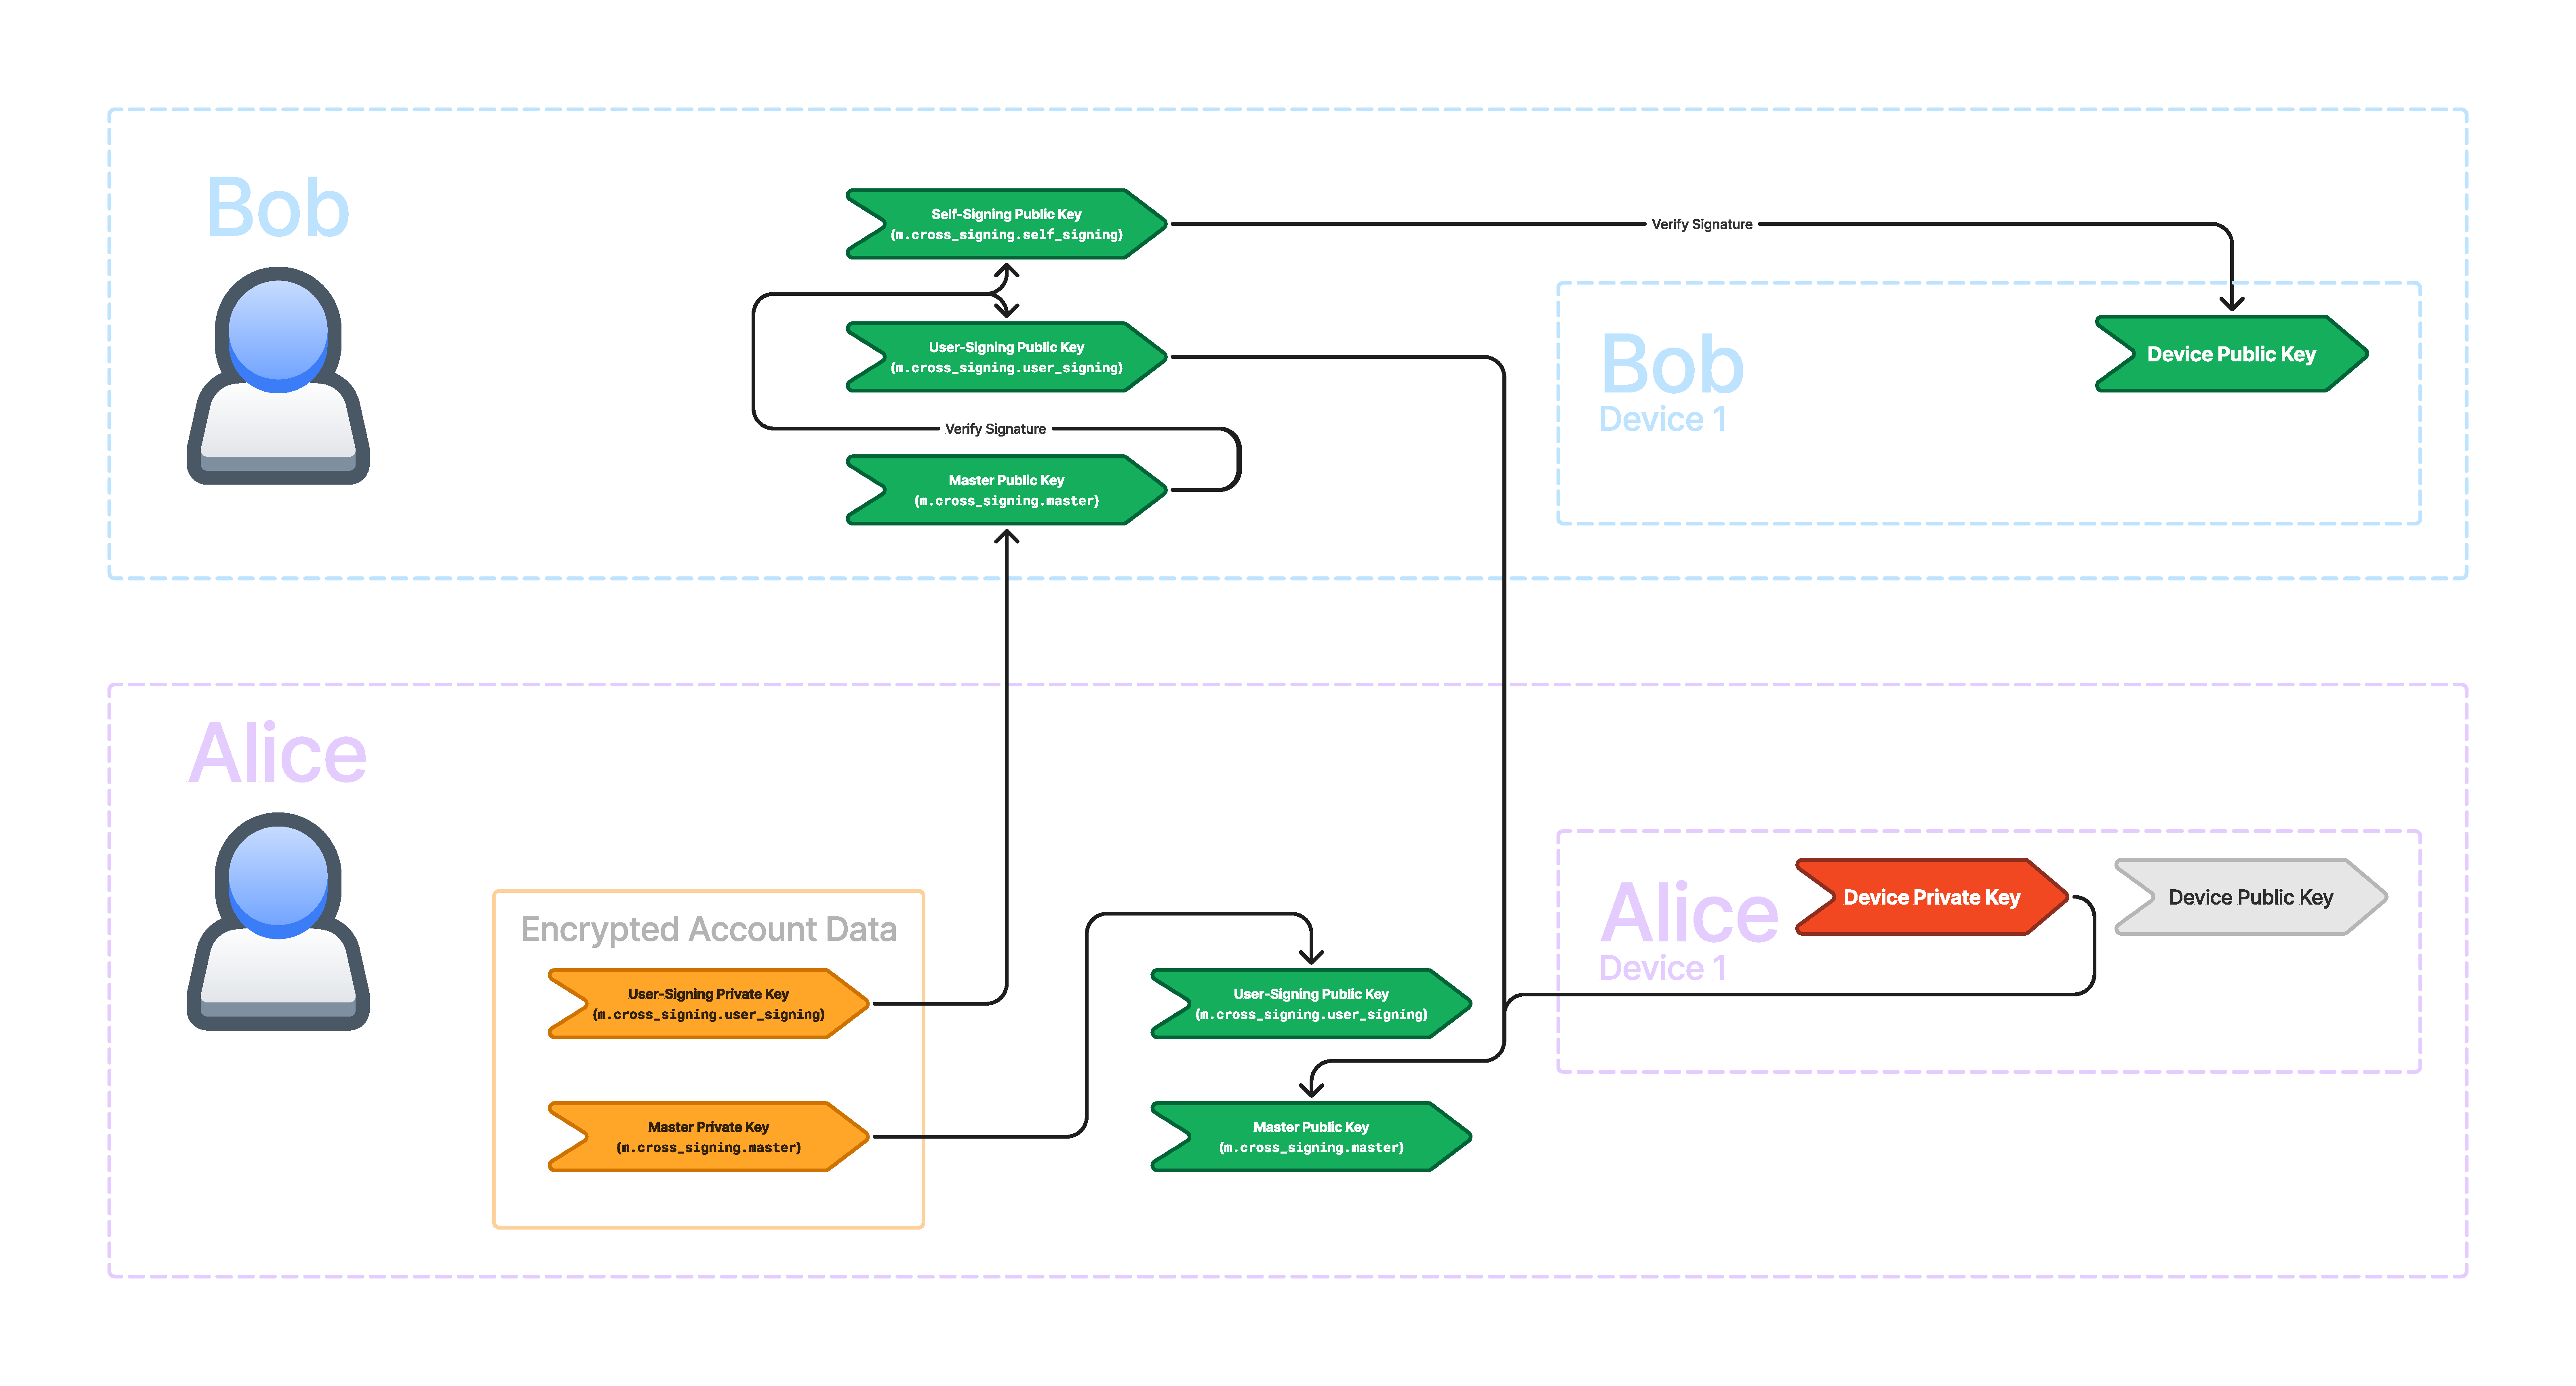
\includegraphics[width=\textwidth]{images/identity-user-verification-zoomed}

    \note[item]{
        The user we want to trust has \textbf{already signed} their devices with
        their \textbf{self-signing key}, which is itself \textbf{signed} by
        their \textbf{master key}. So, if we are able to \textbf{trust their
        master key}, we will have a \textbf{chain of trust} to all of their
        devices.
    }

    \note[item]{
        This is where the \textbf{user-signing key} comes into play. The
        user-signing key \textbf{signs other users' master keys} and is itself
        \textbf{signed} by our \textbf{own master key}.
    }

    \note[item]{
        This creates another \textbf{chain of trust}.

        The \textbf{device private key} signs the \textbf{master public key}
        which corresponds to the \textbf{master private key}.

        The \textbf{master private key} signs the \textbf{user-signing public
        key} which corresponds to the \textbf{user-signing private key}.

        The \textbf{user-signing private key} signs other users' \textbf{master
        public keys}.

        We can \textbf{verify} the signatures by the other user's \textbf{master
        private key} using their \textbf{master public key}.

        Since their \textbf{master private key} signed their \textbf{self-signing
        public key}, we can \textbf{verify} the signature and \textbf{trust}
        their \textbf{self-signing key}.

        Since their \textbf{self-signing private key} signed their \textbf{device
        public keys}, we can \textbf{verify} the signatures and \textbf{trust}
        their \textbf{device keys}.
    }
\end{frame}

\section{Secure Secret Storage and Sharing (SSSS)}
\note{
    Wow, that's a lot of keys! Where are they stored?
}

\begin{frame}{Don't Forget Your Keys}
    \includegraphics[width=\textwidth]{images/overview}

    \note[item]{
        The \textbf{public keys} can be stored on the \textbf{server}.
    }
    \note[item]{
        However, the \textbf{private keys} need to remain in the user's control.
    }

\end{frame}

\begin{frame}{Don't Forget Your Keys}
    \includegraphics[width=\textwidth]{images/secret-keys-highlighted}

    \note[item]{
        Today, we've seen private keys for \textbf{key backup}, \textbf{user
        signing}, and \textbf{device signing} as well as the \textbf{master
        key}.
    }

    \note[item]{
        These keys are \textbf{stored} on \textbf{each} of \textbf{your devices}
        and can be \textbf{shared} with your \textbf{other verified devices}
        using those Olm-encrypted \textbf{to-device} events.
    }

    \note[item]{
        But what if you \textbf{sign out} of all of your devices or \textbf{lose
        access} to them?
    }
\end{frame}

\begin{frame}{Don't Forget Your Keys}
    \includegraphics[width=\textwidth]{images/other-stuff-ssss}

    \note[item]{
        That's where \textbf{secure secret storage and sharing} (also known as
        \textbf{SSSS}, or \textbf{quadruple S}) comes in.
    }
    \note[item]{
        It allows you to \textbf{store} your keys \textbf{encrypted} within
        \textbf{account data} on the \textbf{server}.
    }
    \note[item]{
        Let's zoom in and see what's going on.
    }
\end{frame}

\begin{frame}{Don't Forget Your Keys}
    \includegraphics[width=\textwidth]{images/ssss-zoomed}

    \note[item]{
        The \textbf{key} that SSSS uses to \textbf{encrypt} the account data is
        effectively the \textbf{recovery key}.
    }
    \note[item]{
        There is a \textbf{base58-decode} and an \textbf{HKDF} transformation
        which \textbf{produces} the \textbf{actual key}, but it's basically just
        your \textbf{recovery key} that \textbf{unlocks} the \textbf{encrypted
        account data}.
    }
    \note[item]{
        So, you can probably see that if you \textbf{lose your recovery key},
        and you have \textbf{no signed-in devices}, there is \textbf{no way to
        recover the private keys}. This is why it's important to \textbf{store
        the recovery key in a safe place like a password manager}.
    }

    \note[item]{
        So, what's this \textbf{bottom part?} It's \textbf{not} actually
        \textbf{strictly necessary} for the \textbf{encryption}, but it allows
        you to \textbf{verify} that your \textbf{recovery key} is
        \textbf{correct} before trying to decrypt account data. If you want the
        details here, you can \textbf{read the blog post} associated with this
        talk.
    }
\end{frame}

\begin{frame}{Big Picture}
    \includegraphics[width=\textwidth]{images/overview}

    \note[item]{
        Let's go back once more to the overview.
    }
    \note[item]{
        We've talked about each piece of this diagram.
        \begin{itemize}
            \item We talked about the \textbf{Megolm session}
            \item We talked about \textbf{to-device events}
            \item We talked about \textbf{key backup}
            \item We talked about \textbf{self-signing of devices}
            \item We talked about \textbf{signing of other users}
            \item And then we talked about \textbf{secure secret storage and
                sharing}
        \end{itemize}
    }
    \note[item]{
        I hope that this presentation has helped you \textbf{understand} how it
        \textbf{fits together}.
    }
    \note[item]{
        My \textbf{goal} is to \textbf{convince} people that Matrix
        \textbf{cryptography is not scary}. It's \textbf{complex}, but not
        \textbf{inaccessible}.
    }
    \note[item]{
        If you have \textbf{access} to all of the \textbf{underlying
        cryptography primitives}, all of this is something that a
        \textbf{security-conscious programmer} could \textbf{implement}.
    }
    \note[item]{
        You almost certainly \textbf{should not} implement the
        \textbf{cryptography primitives} yourself, but \textbf{composing} them
        together is doable.
    }
\end{frame}

\begin{frame}{Thank You for Listening!}
    \note[item]{
        And with that, I'd like to \textbf{thank you for listening!}
    }
    \note[item]{
        You can \textbf{scan the QR code} for the \textbf{blog post} associated
        with this talk. The \textbf{slides} are \textbf{available to download}
        there.
    }
    \note[item]{
        \textit{If there is time:} I believe we have a few minutes for
        any questions you may have.
    }
    \note[item]{
        \textit{If there is \textbf{not} time:} It looks like we don't have time
        for questions, but I'm happy to talk to you off-stage about any
        questions you have.
    }

    \center{Questions?}

    \begin{center}
        \includegraphics[width=0.5\textwidth]{images/article-qr}
        \scriptsize
        \href{https://sumnerevans.com/posts/matrix/cryptographic-key-infrastructure}{sumnerevans.com/posts/matrix/cryptographic-key-infrastructure}
    \end{center}
\end{frame}

\end{document}
% Local Variables:
% TeX-command-extra-options: "-shell-escape"
% End:
